The general equation of second degree can be represented as:
\begin{align}
\vec{X}^T\vec{V}\vec{X} + 2\vec{u}^T\vec{X} + f = 0
\end{align}
The above \ref{eq:solutions/40/9/eqn1} can also be written as:
\begin{align}
\vec{X}^T\myvec{55 & -60\\-60 & 20}\vec{X} + 2\myvec{32 & -24}\vec{X} +0 = 0
\end{align}
So, 
\begin{align}
\vec{V} = \myvec{55 & -60\\-60 & 20}
\end{align}
and 
\begin{align}
\vec{u} = \myvec{32 \\ -24}\\
f=0
\end{align}
Now, 
\begin{align}
\det{\vec{V}} = \mydet{55 & -60\\-60 & 20}\\
\implies \det{\vec{V}} = -2500 <0
\end{align}

As $\det{\vec{V}}<0$, so we can say that the above conic section \ref{eq:solutions/40/9/eqn1} is hyperbola.Now,
\begin{align}
\vec{V}^{-1} =\frac{1}{-2500} \myvec{20 & 60\\60 & 55}
\end{align}
The center of this hyperbola will be:
\begin{align}
\vec{c} = - \vec{V}^{-1} \vec{u}\\
\implies \vec{c} = \frac{1}{2500} \myvec{20 & 60\\60 & 55} \myvec{32 \\ -24}\\
\implies \vec{c} = \myvec{-\frac{8}{25} \\ \frac{6}{25}}\\
\end{align}
 Now the characteristic equation of $\vec{V}$ is obtained as:
\begin{align}
\mydet{\vec{V} - \lambda\vec{I}} =0\\
\implies \mydet{55-\lambda & -60\\-60 & 20-\lambda} = 0\\
\implies \lambda^2 - 75\lambda - 2500=0
\end{align}
The eigen values are given by:
\begin{align}
\lambda_1=100\\
\lambda_2 = -25
\end{align}
The eigen vector $\vec{P}$ is defined as:
\begin{align}
\vec{V}\vec{P} = \lambda \vec{P}\\
\implies (\vec{V} -\lambda\vec{I})\vec{P} = \vec{0}
\end{align}
For $\lambda_1$=100,
\begin{align}
(\vec{V} -\lambda_1\vec{I}) = \myvec{-45 & -60\\-60 & -80}
\end{align}
By row reduction,
\begin{align}
\myvec{-45 & -60\\-60 & -80}\xleftrightarrow[R_1\leftarrow R_1 /(-5)]{R_2\leftarrow R_2/(-5)}\\
\myvec{9 & 12\\12 & 16}\xleftrightarrow[R_1\leftarrow R_1 /3]{R_2\leftarrow R_2/4}\\
\myvec{3 & 4\\3 & 4}\xleftrightarrow[]{R_2\leftarrow R_2-R_1}\myvec{3 & 4\\0 & 0}
\end{align}
So, 
\begin{align}
(\vec{V} -\lambda_1\vec{I})\vec{P_1} = \vec{0}\\
\implies \myvec{3 & 4\\0 & 0} \myvec{v_1\\v_2} = \myvec{0\\0}\\
\implies \vec{P_1} = \myvec{-\frac{4}{3}\\1}
\end{align}
Similarly,
For $\lambda_2$=100,
\begin{align}
(\vec{V} -\lambda_2\vec{I}) = \myvec{80 & -60\\-60 & 45}
\end{align}
By row reduction,
\begin{align}
\myvec{80 & -60\\-60 & 45}\xleftrightarrow[R_1\leftarrow R_1 /5]{R_2\leftarrow R_2/5}\\
\myvec{16 & -12\\-12 & 9}\xleftrightarrow[R_1\leftarrow R_1 /4]{R_2\leftarrow R_2/(-3)}\\
\myvec{4 & -3\\4 & -3}\xleftrightarrow[]{R_2\leftarrow R_2-R_1}\myvec{4 & -3\\0 & 0}
\end{align}
So, 
\begin{align}
(\vec{V} -\lambda_2\vec{I})\vec{P_2} = \vec{0}\\
\implies \myvec{4 & -3\\0 & 0} \myvec{v_1\\v_2} = \myvec{0\\0}\\
\implies \vec{P_2} = \myvec{1\\ \frac{4}{3}}
\end{align}
By eigen decomposition $\vec{V}$ can also be written as:
\begin{align}
\vec{V} = \vec{P}\vec{D}\vec{P}^T
\end{align}
where 
\begin{align}
\vec{P} = \myvec{\vec{P_1} & \vec{P_2}}\\
\vec{D} =\myvec{\lambda_1 & 0\\0 & \lambda_2}
\end{align}
So, 
\begin{align}
\vec{P} = \myvec{-\frac{4}{3} & 1\\1 & \frac{4}{3}}\\
\vec{D} =\myvec{100 & 0\\0 & -25}
\end{align}
and 
\begin{align}
\vec{u}^T\vec{V}^{-1}\vec{u}-f=16>0
\end{align}
So, the axes are:
\begin{align}
a=\sqrt{\frac{\vec{u}^T\vec{V}^{-1}\vec{u}-f}{\lambda_1}} = \frac{2}{5}\\
b=\sqrt{\frac{f-\vec{u}^T\vec{V}^{-1}\vec{u}}{\lambda_2}} = \frac{4}{5}
\end{align}
Now, the equation \ref{eq:solutions/40/9/eqn1} can be written as:
\begin{align}
\vec{y}^T\vec{D}\vec{y}=\vec{u}^T\vec{V}^{-1}\vec{u}-f
\end{align}
where, 
\begin{align}
\vec{y}= \vec{P}^T (\vec{x}-\vec{c})
\end{align}
So, 
\begin{align}
\vec{y}^T\myvec{100 & 0\\0 & -25}\vec{y}=16\\
\implies \vec{y}^T\myvec{100 & 0\\0 & -25}\vec{y}-16=0
\end{align}

\begin{figure}[!ht]
\centering
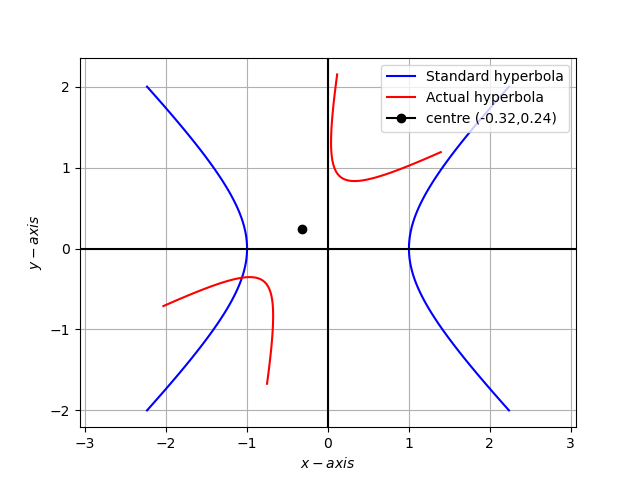
\includegraphics[width=\columnwidth]{./solutions/40/9/figs/hyperbola_2.png}
\caption{Comparison of the Standerd and Actual Hyperbola}
\label{eq:solutions/40/9/fig:hyperbola}
\end{figure}




